\documentclass[12pt]{report}

\usepackage[margin=1.0in]{geometry}

\usepackage{graphicx}
\graphicspath{{./images/}}

\usepackage[
backend=biber,
style=numeric,
sorting=none
]{biblatex}
\addbibresource{references.bib}



% Title Page
\title{Robinson Observatory Telescope Refresh}
\author{Bradley Glaser, Derek McCrae, Bryan Ocbina, Justin Rudisal}


\begin{document}

\maketitle

\begin{abstract}
\end{abstract}

\section*{Executive Summary}
Do what you say you will do.\cite{heinrich}

\section*{Technical Content}

\subsection*{Project Narrative}

The Robinson Observatory is a facility at UCF that is used for both education and research on the topics of astronomy.  It is run by members of the Planetary Sciences Group and the Astronomy Society in the physics department.  The observatory provides high resolutions of astronomical objects and various events and programs involving the UCF and Central Florida to connect members of the community to astronomy .  The main telescope at the observatory is a 20-inch f/8.2 RCOS Ritchey-Chretien telescope and has recently had issues regarding its mobility.  The telescope is able to align itself to a starting reference point, but when given instructions to move to a certain coordinate, the telescope will unreliably move towards the coordinate without any relation to its physical capabilities or location.  This leads to a layer of issues.  The main issue involves being completely off-course of the desired coordinate.  The telescope software will either output warnings too early or too late and not prevent the telescope from colliding with its mount which causes damage to the entire system.  This is a hazard to the staff and the powerful and high cost telescope itself.

The origin of the problem is questioned whether it is a mechanical issue or a problem with the various software that are involved in operating the telescope.  Our computer science team alongside the electrical engineering and mechanical engineering teams will work together to determine the issues and provide solutions that will assist in leading bringing back the telescope to full functionality.  The main concern of the team at the observatory in regards to computer science is that the software of all of the components of the telescope are able to communicate properly on Windows 10.  The components are the telescope, TheSkyX Professional software, the focuser software, and the dome control software.  Meeting this specification will require research into each component of the system and also research into possible software/driver compatibility issues.  The knowledge to code drivers ourselves may be required.  Possible roadblocks may be that certain softwares are not updated or maintained to current standards which would require an overhaul of the system to have all components compatible.  Having the telescope and its surrounding system compatible will be the main objective of our project.

The second objective for our team will be to assist the research opportunities  and community outreach events available at the Robinson Observatory.  Our team will be designing a database capable of storing the images, and their metadata, taken directly by the telescope.  This database will function alongside a user-friendly website that can be used by the community for sharing images and also by the astronomer team to conduct research.  The images will be indexed with their relevant data and a search functionality will be available.  This will provide storage for the data collected at the observatory and assist in long-term research.  On the community side, the website will allow the observatory to easily share images with those interested.  A possible stretch goal is to use machine learning to search images for known objects based on a gathering of previous tagged images of the object.

The third objective will be to assist the electrical engineering team in modeling the black box which serves as the main component for issuing commands to the telescope.  The model will replicate the functionality of the telescope in turns of movement and sending and receiving data.  The current goal for the model is to be able to track the sun or moon within the accuracy of a degree.  This model will assist future teams as the complexity of the black box has been deemed to be too large in scope for a single year senior design team.  The reverse engineering of the black box will be useful for moving away from proprietary systems and give greater control to the team at the observatory in terms of what they would like out of the telescope, making it more programmable to their personal needs.

There are also a series of additional objectives pertaining to recording and storing astronomical data that will be obtained from the software when taking images.  They are outlined in the later sections of this document but serve to either allow for better research opportunities for the astronomer team or to simplify a process and improve the functionality of the facility through accessibility between systems at the observatory or allowing for online access to the faculty or community.

The refresh of the Robinson Observatory is a goal that is extremely important to each member of our team.  This project serves as an opportunity to give back to our university for all the experiences we have gained in our past few years here.  A reminder of all the knowledge we have accumulated into a single project demonstrating our technical skills and problem solving ability.  We hope to be able to remember our senior design project proudly as we bring an end to our time with education and proceed into the professional world of computer science.  Each of our members would also like to address their own personal interests and motivations in this project.

\subsection*{Personal Interest}

\subsubsection*{Justin Rudisal}

My personal interest in this project is twofold with the first part being due to the subject area being space, and the second due to the project area involving a level of mechanical integration. Within my own personal experience with Internships, I have worked heavily with website development and database management. However, I have absolutely no knowledge of mechanical systems and how a computer communicates with a physical, moving part. My dream goal is working in the creative entertainment programming field, such as Universal Creative or Disney Imagineering, and so I need this basic machine programming experience to be successful in my pursuit of a career in those areas.

I also have been in love with space and space exploration for as long as I can remember, and so much so that I originally was planning on doing a double major in both Computer Science and Astronomy until I sadly realized I could not afford to pursue both. So when I heard of the senior design project that would be combining both the area of knowledge that I wish to learn more in with an area of passion that I love, I knew I had to jump on it as quickly as I could.

Other major considerations of mine for this project include the fact that it is a completely open-source undertaking. The end goal of this is to be able to document and demonstrate everything we do so that other small observatories around the world can easily duplicate our results. Projects such as that are the ones that drive my passion in programming, as well as the engineering field in general, because I fully stand behind and support anything with altruistic goals that benefits other people for the common good. I personally believe intellectual progress is achieved from the sharing of knowledge freely, and not from the selling of it for a profit.

I also want to leave a legacy behind me within my university that I have called home for the past handful of years, and that has brought so many different opportunities into my life. I want to give back to the place that has given so much to me. Being able to refresh the telescope and have my name on such a substantial undertaking is one way that I can give back and leave that legacy. I can come back years later, point at the observatory, and say "I helped repair that and bring it into the modern era". Now that is both a great resume builder, and overall achievement to be proud to talk to others about.

I remember one of my most favorite experiences from my first years at college was actually going to the observatory for "Knights Under the Stars" throughout my first few semesters, and being able to watch the telescope work and see the screen show images of our galaxy. I thought that was one of the most fascinating things ever, and it sparked an even bigger passion in astronomy in my life. Lack of time, and it's breaking, caused me to stop going as I got into my higher level classes, but that initial impression left on me caused me to instantly want to help repair the observatory when it was announced as a senior design project.

\subsubsection*{Derek McCrae}

I want to embark on this project primarily for my interest in space. Growing up near the Kennedy Space Center, I was viewing the shuttle launches from a young age and dreamed upon what is out there. A sight I will always want to see firsthand has been strengthened by the pictures provided by telescopes. Telescopes provide a great photos of our universe that can't be currently reached by humans like the Hubble Telescope showcasing the Pillars of Creation or a simple home telescope to view Jupiter. This passion that has grown stronger with the advancements being made for commercial trips to space, especially the advancements by SpaceX. The technological advancements SpaceX has made with getting their boosters to land safely back at a landing pad simultaneously is one of the coolest things I have seen in the last decade. SpaceX along with Virgin Galactic have brought excitement back to space exploration. Some great memories I have include watch parties that had telescope viewings of either a launch, or eclipse, or viewing of another planet.

I had two events that greatly enhanced my passion for space. The first one happened when I was in 7th grade and our class trip was to the Kennedy Space Center. We were able to tour the facilities and sleep under one of the rockets that had on display. The trip helped gain new knowledge and greater appreciation of space. The second event happened freshman summer of high school on a trip to North Carolina. I was family on the side of a mountain in some cabins. One night the mountain staff held a viewing party. My family along with other guests were able to view the stars and use a telescope to see planets only viewable at that time of the year. The event showed me how the topic of space can bring people together.

These two events are a cornerstone to why I wanted to be apart of this project. I know firsthand how viewing parties can bring people together and the knowledge can be beneficial. Not many people own their own personal telescope so this observatory can give those interested a better way to view the sky. To know, I will have a helping hand in allowing activities to once again be performed at the observatory is exciting. The observatory can bring back “Knights Under the Stars” allowing many the current unavailable opportunity of getting to see the stars up close. The observatory could even provide new research study opportunities for those at UCF.

The next reason I chose this project was to build experiences on ideas I have yet to work with. My initial interpretation for this project was a new software needs to be created to help the telescope return to working order. I have learned how to code basic programs and taught programming stepping stones over the past few years without getting any real world experience. I have been eager to apply my knowledge to develop something that will be used past my educational career here at UCF. Furthermore, it will be applying this knowledge to help build something in an industry I am passionate about.

My final motivation for this project is the ability to leave behind a legacy. Of course, the legacy could become poor if this project isn’t completed properly but with proper completion, our solution will outlast my time here at UCF. This refresh could impact this university and space exploration for the next few years and that provides a strong legacy.

\subsubsection*{Bradley Glaser}

I have always had a deep love for everything space. Likewise, my science classes were always some of my favorite courses in school. From a very young age I was always asking questions and some of the biggest unanswered questions are extraterrestrial. The exploration and study of the cosmos must be one of humanity’s priorities if we are to advance as a civilization. I realize that my contributions to the Robinson Observatory are not quite earth shattering. However, I am happy to be able to say that I am a small part of that undertaking.

My father was always a very strong influencer in my life and he has always pushed me to pursue my goals. When I was in elementary, he got me my first childhood telescope. It was one of my most prized possessions. I kept it for many years and I have fond memories of stargazing with my friends and family. This project is an amazing opportunity to work on a full size telescope. One the day that we were assigned the projects, I called my father and told him about my selection. He was over the moon about it. I cannot wait to dig into this project and make it a reality.

My fiance and I have a special connection because of stargazing. When we lived in Utah, some of our earliest dates were spent on the top of a mountain looking at the stars and moon. We would hike up the mountain as the sun went down and then spend our time laying on the ground and watching for shooting stars. Our relationship was built on a shared love of science and space. Space has been a big influence on my life and I hope that my involvement in this project will help others to capture that same magic.

Intellectual property is a big concern of mine. I understand the value of having outside companies come to UCF and pitch projects. Students need real work experience and those businesses are able to provide it. However, the cynical side of me sees these businesses profiting off of the work senior design students are performing for them. Thus, I wanted to choose a project that would be internal to UCF. That way I can be sure that my time spent will not just be putting money into someone else’s coffers.

I wanted to work on a project that was tangible. Many of the projects presented for us to pick from were either esoteric or difficult to explain to non technical persons. Explaining that I will be on the team that fixes UCF’s observatory is immediately easy for anyone to understand. Likewise, I felt that potential employers would be more responsive to a project which was for the immediate betterment of others. It is hard for the average person to understand how “analyzing blockchain correctness” will affect them. However, I am able to point to the telescope and say “you couldn’t visit that before and now it works”. That direct impact is something that I wanted to have for a project.

Being able to contribute to UCF and help future students foster their love of astronomy is a dream come true. I hope that my contributions to this project will help others discover their passions. Similarly, the ability to leave a legacy behind at UCF is a big bonus. Many of the projects presented to us seemed fleeting or shallow in my opinion. They dealt with trivial things that, in the case of blockchain, might not even be relevant in the coming years. I hope that our contributions are more substantial and that they will stand the test of time.

\subsubsection*{Bryan Ocbina}

After hearing the pitch for this project, I realized being able to provide a meaningful impact on the UCF community was significant for myself.  I have grown up in Orlando all my life and have been ingrained to love all thing related to Florida from Disney and mickey mouse to the beaches and manatees to watching rocket and shuttle launches liftoff from Kennedy Space Center, with pure amazement every single time.  As I enter my final year as a Computer Science student, I would like to create a lifelong experience and memory here in my hometown before I finish my education, graduate, and begin to use my knowledge and technical skills in the professional world wherever my career may take me.  Aiding in the Robinson Observatory refresh is a project that aligns with my interests and goals and is my first choice amongst the about fifty projects presented to us.

One of my favorite memories is going on a camping trip a few summers ago and being to stargaze with close to zero light pollution.  The night sky at this time was and is still the most amazing and unforgettable sight I have ever seen.  I had a realization after seeing the sheer number of stars and the surprising amount of color of how much beauty we miss out on living in the city with lights everywhere.  Likewise, as another unforgettable experience was a viewing of a nighttime shuttle launch from my home in Orlando that lit up the sky as if the sun was rising.  Space and the stars above bring out childlike wonder in myself and brings excitement as our team begins to develop our design for the Robinson Observatory refresh.  To be able to once again share images from the telescope at the observatory and hopefully inspire some childlike wonder in someone else is an important part of this undertaking.

The UCF community and Central Florida as a whole is a wonderful center for growth and dreams.  Community outreach is a valuable aspect of this project.  Public events such as “Knights Under the Stars” held at the Robinson Observatory allow for people of all ages to explore the night sky and learn about our solar system and various nearby stars or other celestial phenomenon.  However with the main 20-inch telescope out of commission, the ability to view the night sky at these events is undoubtedly weakened.  We hope to not only restore this functionality but to also add on and allow for images from the 20-inch telescope to be shared more easily with the community.

As another part of community outreach, a decisive part of joining this project includes the open-source aspect of working with UCF.  This project serves to better the research opportunities available locally in Central Florida and our work done with the observatory will not be used to profit some business’s latest product.  The story of the project is much more involved and personal than the other projects pitched to our class.  We are able to not just present a fleshed out, functional telescope as a project we worked on but as an entire experience that could serve to inspire a future astronomer, aerospace engineer, or astronaut.

This project will be my number one priority for my remaining time as a student and I hope to gain as much as I can while working with everyone at the observatory and the other student teams as we share our experiences of our different fields and do our best to create an unforgettable experience.  Altogether, the Robinson Observatory refresh project serves as a platform to express my sincere appreciation for my hometown Orlando, Florida. I have many hopes for my senior design team that we will be able to accomplish some amazing features that will modernize the observatory and that will be used and remembered for many years after we have all graduated.  To be able to come back home, visit the observatory, and tell others that I worked on this feature or component at the Robinson Observatory would be a wondrous feeling.

\subsection*{Broader Impacts}

Getting the telescope and observatory working will help with both the different organizations that contract out the observatory for their own scientific pursuits, as well as enhancing its ability to reach out to students and the surrounding community with an accessible means to the stars. Even those who are not local will be able to benefit from this project due to one of our goals being to create an online public viewing platform for what the observatory is currently observing and completing. This opens it up to anyone with access to an online device to actively engage with the observatory, as well as the scientific space community at large. Our goal is to create both an online portal for the observatories sponsors to access the device, as well as crafting a learning environment for everyone.

This online outreach will also help spearhead engagement within space exploration and space overall within STEM groups both in the university as well as local elementary, middle, and high schools. Teachers will be able to pull up the current observatory pictures and developments, and will also be able to speak on weekly events that the observatory will be hosting. The overall goal is to both repair the observatory and bring it up to operating standards, as well as revamping its public outreach through new websites.

The organization that runs the observatory, Florida Space Institute, is a research group that is funded completely off of scientific grants and personal donations. By repairing this observatory for the Florida Space Institute we are helping an organization that may otherwise have a tough time affording the hiring of professionals to accomplish the intended goals. We are also helping to free up the time of those within the organization who may have had to spend their own time figuring out complicated temporary workarounds for the observatories problems instead of doing the scientific work that they want to accomplish.

\section*{Requirements}

The CS team and engineering teams must coordinate together to solve many of the issues currently preventing the telescope from functioning properly. Thus, our project is unique in that some of our requirements might be solved by students from other teams working in parallel to us. Regardless of whichever team solves the problem, we will need to complete all of the requirements specified by FSI.
At the time of completing this document, FSI has not rendered up to date requirements for the scale model solution. Thus, these are the most current requirements. However, the CS team requirements are unlikely to be significantly altered.

\subsection*{CS Team Specific Requirements}

\subsubsection*{Essential Requirements}

The current control computer is running Windows 7. FSI would like the control computer to be upgraded to Windows 10. This presents several challenges. Firstly, we must ensure that “The SkyX Professional” control software is compatible with Windows 10. Likewise, there are several subsystems for controlling the mount, dome, focuser, and camera that must also be compatible with Windows 10. Similarly, the drivers required for the hardware components must be audited to determine compatibility and possibly replaced.

The telescope is currently controlled by a microcontroller “black box” attached to the mount. The CS team must ensure that any upgrades are able to communicate with said box. It is possible that the box might be replaced at some point in the future. Thus, it is important that the CS team understands and documents what signals are transmitted from the control computer to said box.

\subsubsection*{Secondary Requirements}

There is an iMac computer located on the lower level of the observatory. It would be nice if the observatory operators could control the telescope remotely from said computer. Investigating if a virtual machine or remote desktop software will be essential before we begin implementation. The sponsor seemed amenable to a remote desktop solution in order to reduce the number of computers directly controlling the telescope.

Setup a backup server at the observatory to store information gathered by the telescope. They currently have a server in the observatory but they do not know to what degree it is functional nor how the data is stored. We must investigate how it operates and possibly revamp their existing archive system.

Set up a online feed for sharing the most recent data capture by the telescope. As part of a community outreach effort, it would be nice if the public could easily view and interact with the photos generated by the telescope. We would have to convert the scientific specific files generated by the control computer into a publically digestible format.

Increase the accuracy of the control computer’s internal clock. At current, the observatory team is unable to perform certain time sensitive experiments due to the inaccuracy of the computer’s timekeeping. We must determine if the internal Windows method of synching the time can be overridden with a more accurate source.

\subsubsection*{Stretch Requirements}

The CS team would need to investigate the scripting capability of the existing control software. The observatory team had previously indicated that “The SkyX Professional” control software has the capacity to be extended/augmented via an existing scripting plugin. The CS team would need to investigate said system and determine the capabilities. The observatory team indicated that they may want basic functions automated if we have time.

\subsection*{General Requirements}

The dome subsystem needs to be controlled by the computer and integrate with the movement of the telescope. As the control software issues commands to the telescope controller, it must also issue corresponding commands to the dome subsystem. These components must both work in tandem or we will be capturing images of the inside of the dome instead of the stars.

The camera subsystem must be fully functional. Like the dome subsystem, it must communicate with the control software. The temperature, fan control, and camera calibration must be configurable and controllable. Finally, we must be able to accurately set the metainfo in the generated FITS file header generated by the control software.

The focuser subsystem will be a necessary part of capturing viable astronomical images which are fit for general consumption. It will need to be able to directly control the telescope’s focus from an integrated GUI. Likewise, the sponsor would like us to investigate the possibility of optimizing the autofocus routine. Finally, temperature fluctuations can impact the quality of images captured by the telescope. Temperature monitoring might be an option to automatically adjust the telescope focus to compensate for associated fluctuations.

The telescope subsystem controls the physical movements of the hardware. The control software must be able to execute the home and park capabilities of the telescope. Likewise, the control software must be able to send commands to the RA and Dec motors; the slew rates must be set in the control software. The telescope must be able to work in multiple modes. The first mode required is the sidereal tracking mode. Sidereal tracking mode fixes the signal going to the Dec motor, preventing it from moving, and only moves the RA motor tracks at sidereal rate. The second mode is the non-sidereal tracking mode. In the non-sidereal tracking mode both motors are moving at non-standard tracking rates. One area that the CS team needs to investigate is how the existing control software (The SkyX Professional) quantifies the non-sidereal rates. Likewise, we must investigate what units the software uses for said rates. Likewise, the telescope must be controllable manually by an operator directly. This performed via the use of an attached joystick and via the control software itself. At current, in the event of control failure, the telescope is in danger of damaging the both itself and the support infrastructure surrounding the telescope. This problem must be corrected with the use of pointing limits via the use of either physical limits or the control software. Finally, we must establish flip zone parameters near HA=0.

The filter subsystem controls the filters for the telescope. The filters are situated within the camera housing. The filter wheels get the power needed for operation from the camera subsystem. It is worth noting that the observatory has another filter wheel that is not currently connected to the telescope. We must be able to switch filters from within the control software. Research is required to determine if The SkyX Professional supports this operation natively or if we will need to plug into the control software’s scripting system to enable it manually.

\subsection*{Unofficial requirements}

We originally assumed that the telescope could be brought to a working state by the end of the semester. However, the electrical engineering team is unable to analyze and reproduce the necessary hardware in the span of a single senior design project. Thus our electrical engineering comrades will be replicating the motion of the telescope via a scale model. Their team (and possibly the mechanical engineering team) will develop a model which will be able to track celestial bodies in real time. Studying the movements of the model will help them better understand what an eventual solution to the telescope will entail. Thus, it will be one of the CS team’s responsibilities to create the software needed to track said celestial bodies as they pass across the sky. This tracking software will also need to be able to send instructions to the model so that it maintains a fix upon whatever celestial body is chosen. The CS team will be able to utilize the scale model to simulate inputs into any potential archiving software we will develop for the project.

\section*{Ideas}

Our first priority is coordinating with the interdisciplinary teams. Before any of the computer science team components can come to fruition, we must have a functional telescope to generate photos and associated data. Proper calibration and operation is the most immediate concern for our team. A study of “The SkyX Professional” software must be performed before we can assess what factors might be contributing to the current state of nonfunction. Likewise, it is possible that the issues currently plaguing the telescope might be a combination of many factors. Either way, the CS team must be prepared to coordinate and implement solutions in tandem with our engineering counterparts.

A community outreach website which would include both the existing data taken from the current Robinson Observatory website and a live/archived data component. The public data component would enable the public at large to have access to the data gathered by the observatory. Photos and positioning data would be presented to users when they access the website and it would be updated in near real time. As the telescope is operated, data gathered would be immediately available for public consumption. This functionality would have the ability to be enabled/disabled depending on the confidentiality requirements of the current research being done.

The current state of the telescope shows that it is able to calibrate to a reference point of Polaris, the North Star, but has no understanding of its position upon attempting to move to any other location.  A problem occurs when the telescope does not recognize it is reaching its mechanical movement limits to prevent damage to the telescope itself.  A possible solution consists of creating an emergency stop by coordinating with the other engineering teams and developing a functionality to have an emergency stop beyond currently pulling the plug to the motors.  There are some issues to consider when creating this as the telescope is very heavy and has many fragile components.  Moving the telescope requires a ramping up of speed and a deceleration time before coming to a complete stop.  This function would be useful for any hazardous conditions even when the telescope is properly functional. 

Research is an important role at the Robinson Observatory.  The requirements for images and data to be accepted by the global astronomy community demand highly precise timings of exactly when the image is taken.  The telescope currently experiences issues with the timing requirement.  To solve this issue, we would like to be able to create some software that can accurately sync to an atomic clock and output the timing to the telescope image data.  This would provide the accurate timings required and allow for better research opportunities.  Another possibility would be to better the timing of the computer themselves to allow for the system to be more accurate.

Additionally there are servers at the Robinson Observatory that were previously used to store the data gathered from the telescope images. Their current state is not well maintained but we have been made aware that they do start up. Bringing back the servers to functionality would assist in research opportunities for the observatory while also creating a lasting system that could serve as storage for both long-term research and records. A fallback in case the servers are too damaged or unreliable would be to send the backup images to an offsite hosted server either as part of the UCF senior design hosting or to utilize a cloud storage solution. By collecting all of the photos in one place, we will be able to categorize them and make them more accessible to the researchers. Likewise, we might be able to generate new insights into their data via the use of machine learning. The ability to find patterns in existing data could open new avenues for future research to take place. In order to accomplish any meaningful machine learning, we must ascertain what types of research the existing staff does with their data, what their workflows are like, and how we can improve upon their methods with the application of computer science.

As the Robinson Observatory already has many chances for educational events, additional software or programs that would assist at these events would prove to be useful.  One idea is to provide quiz templates for information related to images capture by the telescope such as identifying astronomical objects ranging from planets, comets, stars, galaxies, etc.  There are many opportunities to provide additional activities at events such as Knights Under the Stars.  

A possibility of being able to view images provided by the telescope in augmented reality at and around the observatory with simple description when interacting with the astronomical objects provides another technological experience for community members and to get more people interested in space and astronomy.  Interaction stations could be tied to GPS coordinates and provide short descriptions or quizzes at each station.  Some kind of reward for answering correctly and learning such as additional images from the telescope that players could keep.  

Image analysis and machine learning for the observatory to be able to recognize various astronomical objects without having to specifically search and point at an object.  Space is full of objects and to be able to identify them quickly would be helpful for research and data collection overall.  This functionality would also serve to allow to automate processes for research by allowing long exposures of specific sections of the sky to be observed over a period of time for any anomalies or changes with known objects.  

The addition of operating the observatory without someone at the facility could be useful to the observatory staff. To implement this feature, we have discussed using scripting and/or an application. Scripting was a feature the observatory once had so we could fix and build off that. Scripting would be the safest choice as no one could gain improper access to the telescope through an internet application. Scripting would allow someone to write a program that operates the observatory and t would be executed at a future set time. The other way for remote control would be through an internet application. The application would allow the user through proper verification to remotely control the observatory.

\section*{Budget}

\subsection*{Software}
The SkyX Professional Access: \$349.00 - Already Downloaded\\
Windows 10: \$140

\subsection*{Web \& App Development}
Web Server Hosting - AWS - use of student credits and free tier limits negate cost\\
Database - AWS - use of student credits and free tier limits negate cost

\subsection*{Physical Hardware}

Data storage cost for backing up the disk image - FSI provided hard drive\\
Physical Server - Observatory already has server




\begin{figure}
	\section*{Block Diagrams}
	\centering
	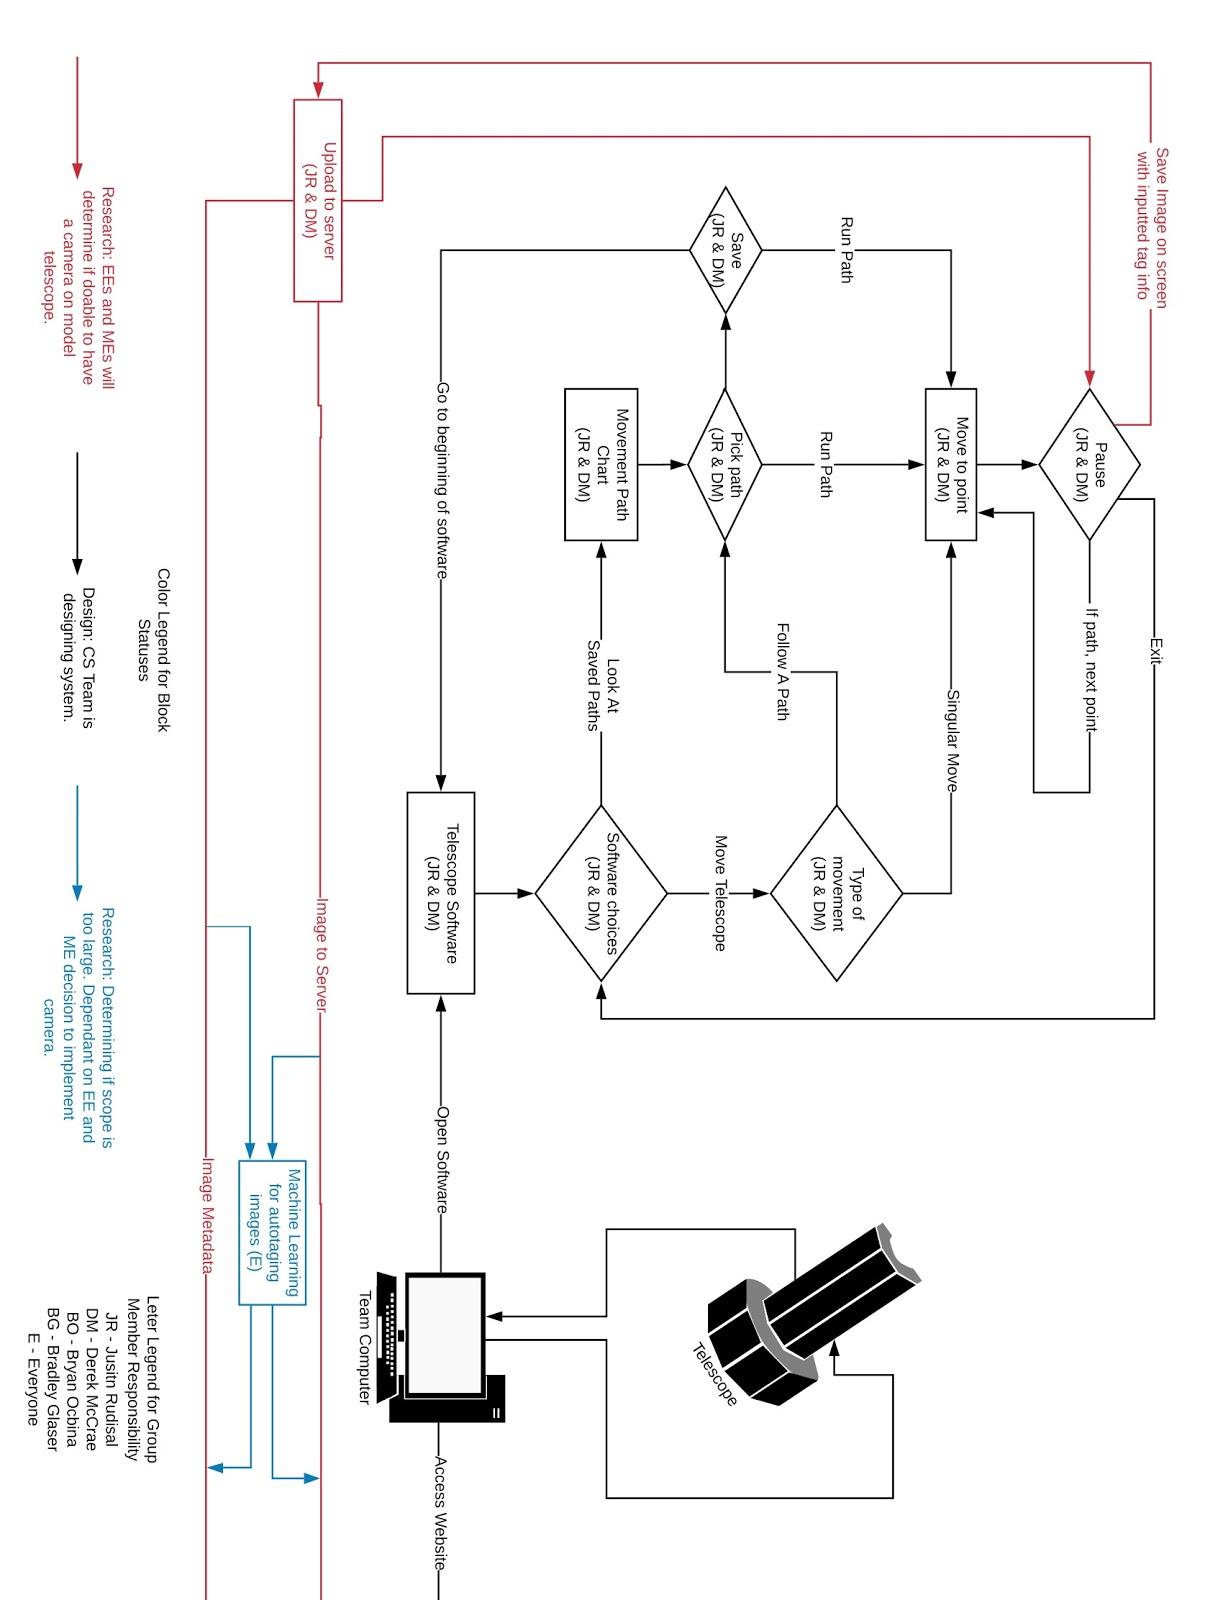
\includegraphics[height=\textheight,width=\linewidth]{blockpt2}
\end{figure}

\begin{figure}
	\centering
	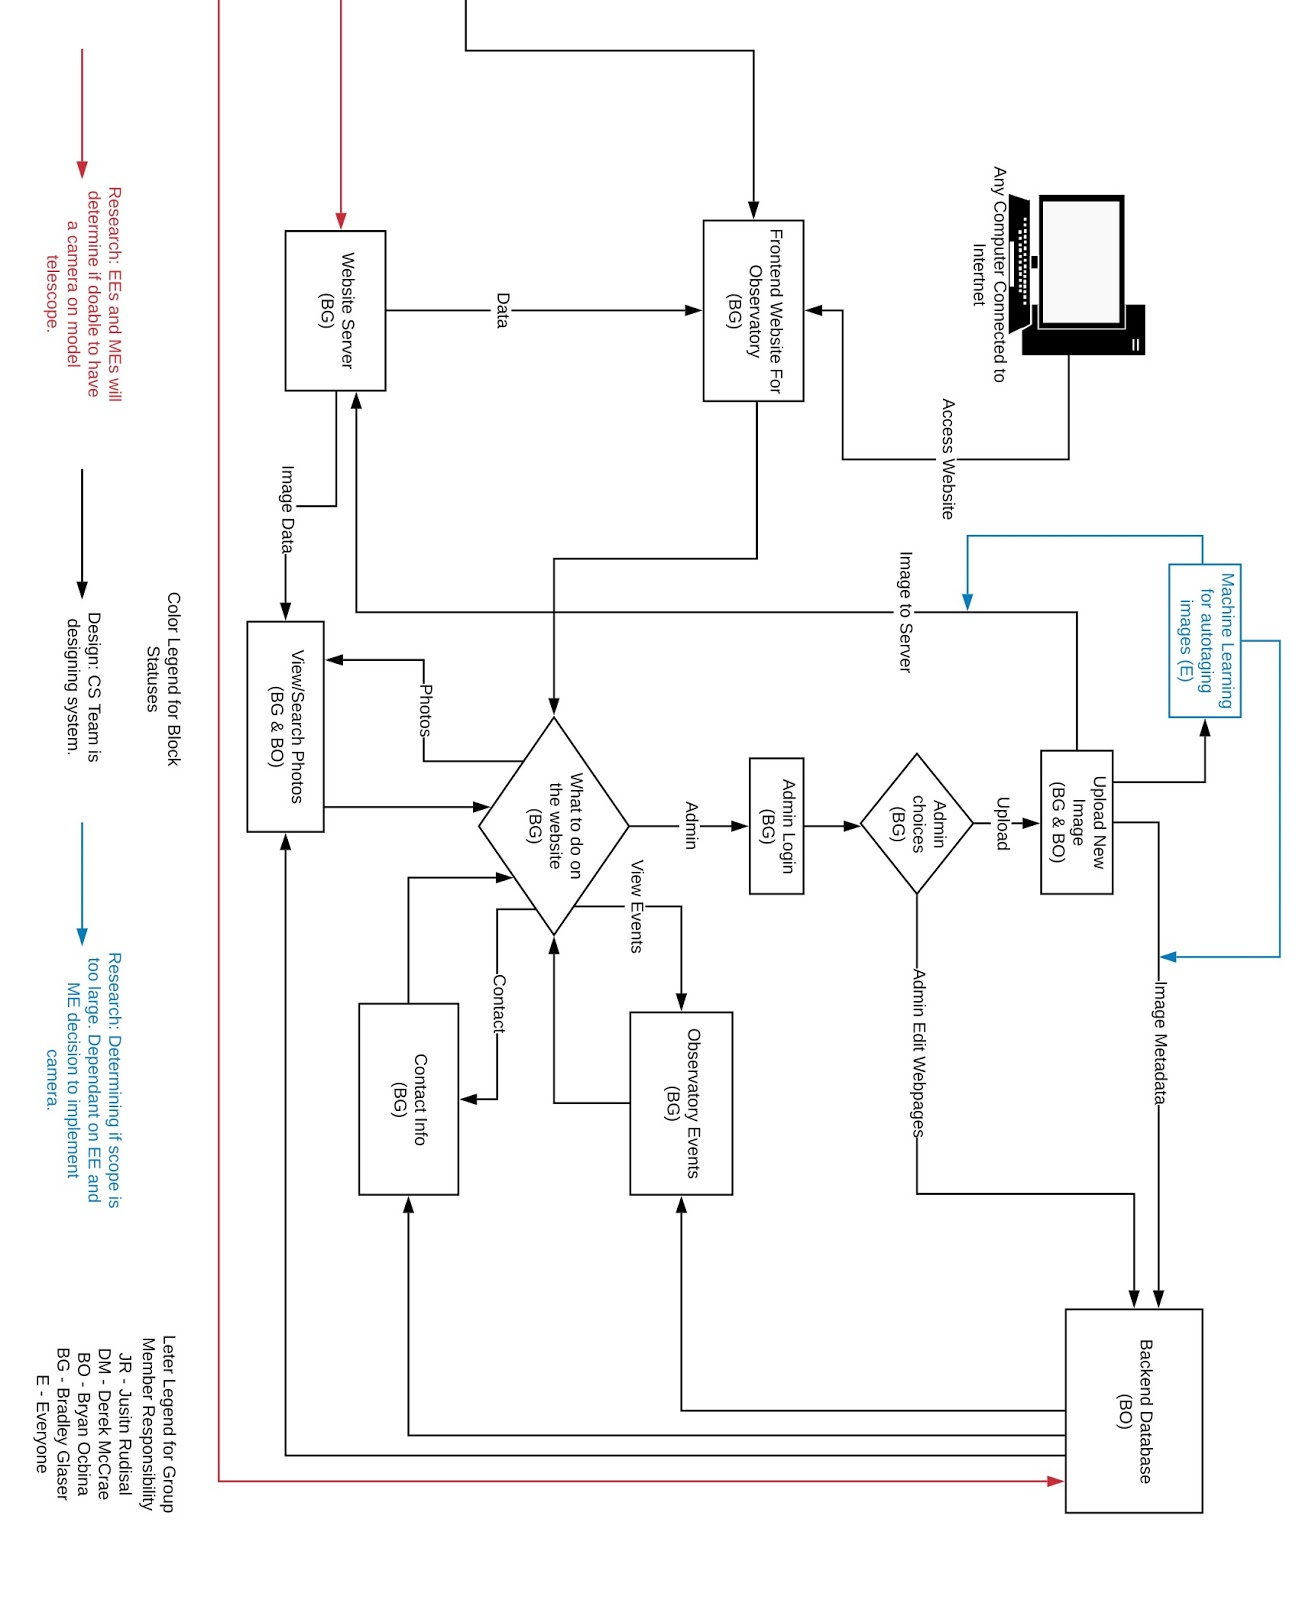
\includegraphics[height=\textheight,width=\linewidth]{blockpt1}
\end{figure}

\newpage %Page break

\begin{figure}
	\section*{Project Milestones SD1}
	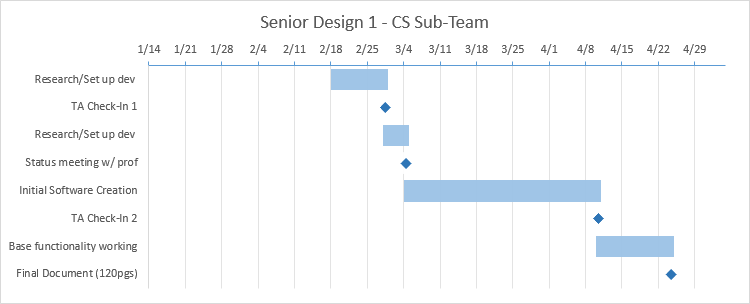
\includegraphics[width=\linewidth]{SD1Gantt}
\end{figure}

\begin{figure}
	\centering
	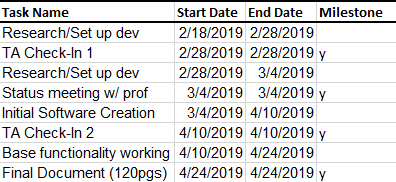
\includegraphics{SD1Dates}
\end{figure}

\clearpage

\begin{figure}
	\section*{Project Milestones SD2}
	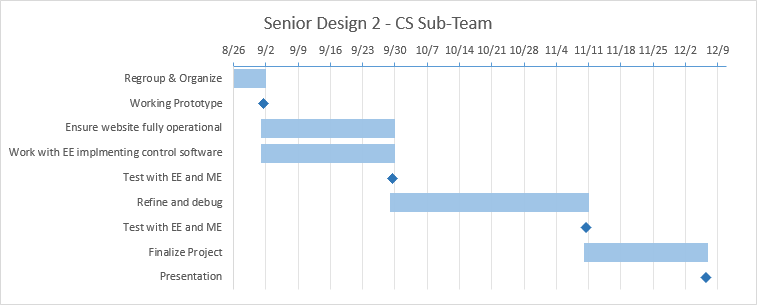
\includegraphics[width=\linewidth]{SD2Gantt}
\end{figure}

\begin{figure}
	\centering
	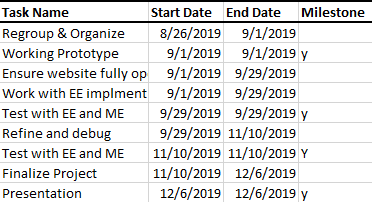
\includegraphics{SD2Dates}
\end{figure}

\clearpage

\section*{Archive Frontend}

The data gathered by the telescope will need to be accessible by future researchers. Likewise, it might be possible to allow the general public to have access to the data. Either way, the data archive will require a frontend to enable browsing, searching, uploading, downloading, and categorizing the data. The frontend will be a login secured website in order to maximize portability and accessibility. By foregoing a native application, we ensure that the data will be accessible from anywhere with an internet connection. Likewise, we enable the researchers to utilize whatever person computers are most convenient. i.e. laptops, a tablet, an iPad, a cell phone, etc.

\subsection*{Frontend Frameworks}

There are many modern frontend frameworks which enable developers to quickly create highly interactive websites efficiently. Our frontend solution will need to be data efficient to reduce the strain on potentially poor connections. It is possible that potential users will have a poor internet connection while attempting to access the data. (As is the case in some observatories.) Thus it is necessary to choose the appropriate framework solution which enables rapid development while maintaining a focus on efficiency.

\subsubsection*{Angular}

The Angular web framework was released by Google in September of 2016.\cite{angularrelease} Angular (also known as Angular 2) was released as a replacement for Angular 1. Its release focused on "a wide range of use cases,...[optimization] for developer productivity, small payload size, and performance."\cite{angularrelease} The framework was built from the beginning via "collaboration with the open source development community."\cite{angularrelease} Thus it has received input from many different developers to ensure that it is flexible enough for general use.

Angular utilizes TypeScript as its implementation language which helps reduce bugs associated with loose typing. Typescript also brings many features absent from plain JavaScript which can help to reduce developer time. Utilizing a framework which already utilizes TypeScript will be more advantageous than trying to use it with a framework which was not built to support it.

Angular is built utilizing component objects. The Angular official quick start guide states that "components are the fundamental building blocks of Angular applications."\cite{angularquickstart} These components "display data on the screen, listen for user input, and take action based on that input."\cite{angularquickstart} Components are a good way of breaking one's code up into reusable pieces. By compartmentalizing one's code in this way, there is a reduction in the duplication of effort. Likewise, it creates the opportunity to test each component separately from the rest of the overall application.

Angular is a good candidate for our archive frontend. It was designed to be extremely flexible. Likewise, it is a commonly used industry frontend framework. Employers look for candidates with existing knowledge of frameworks. Thus it would be useful for our team to gain experience using such a common library.

\subsubsection*{Bootstrap}

Bootstrap is an open-source framework originally developed at Twitter in 2010.\cite{bootstrapabout} It was originally a closed-source tool for internal use at Twitter. However, it was eventually open-sourced due to its popularity with the internal Twitter developers. Twitter found that "developers of all skill levels [could jump] in without any external guidance."\cite{bootstrapabout}

Like Angular, Bootstrap also includes components. However, the Bootstrap components are focused on the display of data and abstains from opinions about the structure of one's data. This decoupled nature means that utilizing components ensures that applications built with Bootstrap share a common look and feel. Familiar components ensure that potential users are quick to acclimate.

Unlike other frameworks, Bootstrap relies on jQuery to handle its JavaScript integration.\cite{bootstrapjs} Thus, Bootstrap is much less opinionated on the frontend code structure. This enables developers to create their own code idioms and integrate into existing code bases easily.

Bootstrap's flexibility is both a strength and a weakness. Experienced JavaScript developers will find said flexibility very useful and will be able to structure their code in a familiar fashion. However, our team lacks experience building frontend web applications. Thus, an opinionated framework may become an initial disadvantage. Other frameworks provide a standard way of structuring code and therefore might be more friendly for our team to work with.

\subsubsection*{Ember}

Ember was a JavaScript frontend library released to compete with Backbone.js, SproutCore, Cappuccino, and Dojo.\cite{emberrelease} Many Ember's original competitors have fallen out of the public eye since its release in August of 2012, yet Ember still sees wide adoption even today. Ember was a departure from aforementioned "microlibrary" competitors that were popular at the time of its launch. Ember was different because it focused on "helping developers grapple with the complexity of building 100\% JavaScript web applications."\cite{emberrelease} They did so by "[embracing] the tools that [web developers] were most comfortable with: HTML and CSS."\cite{emberrelease} Thus, Ember was created as an opinionated JavaScript framework which "[helps] you architect large, multi-page applications, but [helps] you to do so without breaking the basic building blocks of the web."\cite{emberrelease}

When a user visits an individual URL in an Ember application the response is handled via an Ember "route".\cite{emberrouting} Routes are how a developer compartmentalizes pieces of their application functionality into reusable components. Thus, it is important to separate one's application based on functionality to ensure that effort is not duplicated among several different routes. Like the other aforementioned frameworks, Ember enables the developer to test individual components by splitting them up into routes.

Ember decouples data from the display routes via objects called "models".\cite{embermodel} Models are a way to adapt the Ember routes to the application's individual data concerns. Thus, Ember provides strong opinions about how one should structure the application's data.

Ember's focus on preserving web browser functionality is definitely an advantage when compared to some frameworks that may cause something as simple as the back button to function incorrectly. Likewise, its opinionated framework style ensures that our team will have a good idea of how to structure our application. However, Ember's rigid structure might be too strict for our purposes. Our team has compartmentalized the web application into frontend and backend sub-teams. Thus, the frontend team needs to be flexible enough to accommodate however the backend structures their data before the frontend interacts with it.

\subsubsection*{React}

React was a Framework developed by Jordan Walke at Facebook. It was originally a propriety framework that they used internally. However, it was later released as an open-source framework at JSConf US.\cite{reactlaunch} It was released in 2013 and thus it is a relatively new framework in the JavaScript ecosystem.\cite{reactlaunch} However, it has seen high adoption rates among developers.

React is a single-page web application framework. It enables the developer to dynamically update the contents of a page as data changes or uses interact. Since the web browser doesn't have to load completely new pages with each action, the resultant web application is very responsive since it only downloads information as it is needed without the need to potentially re-download components repeated on each page.

Components are React's way of splitting your application into reusable pieces. Likewise, Components determine how one structures the data on the user's end. React components "[take] in parameters...and [they return] a hierarchy of views to display."\cite{reacttutorial} The data is tightly coupled to the visual model.

React's structure and idioms are a good contender for implementation in our project. The single-page nature of React makes it ideal for places with low-bandwidth connections such as observatories. Likewise, the tight coupling of data and view provides a good starting point for structuring our code. Finally, React is widely used in the industry and so it would be an advantage for our team to gain experience using it.

\subsubsection*{Vue}

Vue was released by Evan You in 2014 as an open-source JavaScript frontend framework.\cite{vuelaunch} It received immediate attention from various web communities and it has developed significantly since its launch. It is being actively developed and receives regular bug-fixes and stability patches. Despite its relative immaturity, the framework has seen wide adoption due to its progressive design philosophy.

Vue is compartmentalized across several different libraries. The core library "is focused on the view layer only, and is easy to pick up and integrate with other libraries or existing projects." \cite{vueguide} However, Vue optionally has the capability to "[power] sophisticated Single-Page Applications when used in combination with modern tooling and supporting libraries."\cite{vueguide} Vue's flexibility enables it to integrate into many differing use-cases.

Like the other libraries examined, Vue also supports component composition via Vue's component system. This abstraction system is "an abstraction that allows us to build large-scale applications composed of small, self-contained, and often reusable components."\cite{vueguide} They can be nested and pass data from parent to child. Data passing is done via props and a specialized binding syntax.

Utilizing Vue for our project would mean depending on a relatively immature library. However, its lightweight molecularity will enable us to only utilize the components that we need for our project. By doing so, we will reduce both the complexity of our resultant application and the bandwidth requirements associated with loading the libraries. Likewise, the single-page application nature of Vue will also reduce the amount of data being utilized.

\section*{Model Telescope Control}

\subsection*{Model Telescope vs Observatory Control}

The underlying premise that drives the need for our model telescope is to replicate the control structure that the Robinson Observatory currently has in a scaled-down and testable environment. The observatory is currently controlled by a software and hardware system known as SkyX Professional, which is a commonly used product for small observatories around the globe that helps individuals get their observatory telescopes operating to their fullest extent. However, while this software is extremely useful for the observatories purposes, it is actually a hindrance for our scale model. SkyX Professional does not translate well when being adapted to small-scale custom designed telescopes. By our understanding based on documentation, as well as the physical systems currently in the Robinson observatory itself, the software has a required hardware integration to use the SkyX software for the purposes of controlling the observatory. 

To further explain, this hardware integration is not designed to be used with telescopes that have been fully planned and created from scratch. The main issue lies in that a custom telescope would have its own custom inputs and outputs based on the needs of the creator, while SkyX and its hardware is designed to integrate with well-established brands and models. The actual SkyX software and what it’s sending out and receiving form the observatory telescope is hidden behind a layer of proprietary silence, and so therein lies the need for a custom model telescope control system. We cannot use SkyX as the observatory currently uses it because we are unable to tell what the software and hardware are communicating to each other beyond our reasoning of what we think it might be sending. 

\subsection*{Designing the Model Telescope Control Environment}

With the realization that we could not go the SkyX Professional route for our model telescope also came the realization that we would have to create our own custom telescope control software from scratch. Before doing any further research into what our software will do and how it will function, we first established as a team that this custom software will be open-source and easily transferable from our scale-model telescope to any real telescope. The idea behind this is that we want to be able to take our software and have senior design teams after us be able to use it as a well-defined base for repairing the Robinson Observatory. The entire thought-process behind the scale model to begin with is due to that fact that there is no currently established base, and so our team has no reference form which to repair the observatory ourselves as it stands. 

After some brainstorming and hashing around ideas, our team established that there would be little difference between our model telescope and a robot. In fact, our telescope would essentially be a controllable robot. With this in mind, we realized that we needed to establish a base software from which to do this controlling from. Taking the stance of this being a robot, we are now also free to design and program entirely within a simulator environment to ensure our software will actually work with the physical custom model telescope.  

\subsection*{ROS Integration with Stand-Alone Gazebo}

\subsubsection*{What is Ros?}

The Robot Operating System, otherwise referred to as ROS, is a flexible framework used for the purposes of writing software for robotic systems. It is a collection of tools, libraries, and conventions that aim to simplify the task of creating complex and robust robot behavior across a wide variety of robotic platforms.\cite{ROSDescription} It is commonly used in conjunction with Python and C++. Furthermore, ROS is home to a large community of user-contributed packages that adds a lot of value to integrating ROS into our core systems. Why reinvent the wheel and rediscover wood when we can instead invent a brand new cart from existing discoveries? 

The core of ROS is licensed under the standard three-clause BSD license. This is a very permissive open license that allows for reuse in commercial and closed source products. This works great for the purposes of our model telescope, because we wish to keep our creation entirely open-sourced. While the core parts of ROS are specified as being licensed under the BSD license, other licenses are commonly used in the user-contributed community packages such as the Apache 2.0 license, the GPL license, the MIT license, and even proprietary licenses. For the sake of our aforementioned open-source goal, our team will avoid any community packages that state the use of proprietary licences. Every user-contributed package is required to explicitly state what kind of licensing it uses, and so this should not be an issue for our team. 

\subsubsection*{What is Gazebo?}

Gazebo is a 3D dynamic simulator with the ability to accurately and efficiently simulate robotic systems in complex indoor and outdoor environments. While it appears to be similar to game engines, the differences in Gazebo lies in its ability to offer physics simulations at a much higher degree of fidelity, a suite of sensors, and interfaces for both users and programs.\cite{GazeboDescription} Other key features of Gazebo include multiple physics engines, a vast library of robotic models and environments, and advantageous programmatic and graphical interfaces. This will help create a more conductive programming environment for our team so that we can feel confident in what we create. 

Using Gazebo with our project gives us the ability to rapidly test algorithms in a simulation environment, design our model telescope with the understanding that it is a robot, perform regression testing, and possibly even train our model telescope to use a basic AI system that uses realistic scenarios. To accomplish all of this, Gazebo was designed to work on Linux operating systems and it works the best on Ubuntu, which is a flavor of Linux. Thus, this will require us to install Ubuntu in order to run Gazebo. 

\subsubsection*{Integrating ROS with Gazebo}
To successfully achieve a ROS integration with stand-alone Gazebo, a set of ROS packages named "gazebo ros pkgs", provided by Gazebo, provides wrappers around the stand-alone version of Gazebo.\cite{GazeboRosIntegration} They provide the necessary interfaces to simulate a robot in Gazebo using ROS messages, services and dynamic reconfiguration. 

\printbibliography[title={References}]

\end{document}
